% ============================================================
% RevEdit —— CSCloud 2026 投稿主文件（IEEE 会议模板，6-7 页含参考文献）
% 编译：pdflatex main（参考文献为内嵌 thebibliography，跑两遍更新交叉引用）
% 数据更新：只改 macros.tex；\TODO 标注项等待补漏队列完成
% ============================================================
\documentclass[conference,10pt]{IEEEtran}
\IEEEoverridecommandlockouts
\usepackage{cite}
\usepackage{amsmath,amssymb,amsfonts}
\usepackage{graphicx}
\usepackage{booktabs}
\usepackage{multirow}
\usepackage{xcolor}
\usepackage{tikz}
\usetikzlibrary{arrows.meta,positioning,fit,backgrounds}
\usepackage[hidelinks]{hyperref}
\usepackage{balance}  % 平衡末页双栏
% ============================================================
% macros.tex —— 全部实验数值集中定义，数据更新只改这里
% 标注 TODO 的宏等待 fill-gaps 队列（agnews FT 扫描/密钥压缩×3/
% LLaMA 循环/变体/双水印重测）完成后填充
% ============================================================
\newcommand{\TODO}[1]{\textcolor{red}{[TODO: #1]}}

% ---------- 模型与任务 ----------
\newcommand{\gptwoxlm}{GPT-2 XL (1.5B)}
\newcommand{\llamasevenb}{LLaMA-2-7B}
\newcommand{\nseeds}{3}

% ---------- Table 1: 水印质量 + 密钥移除（mean±std, \nseeds seeds）----------
% 格式: WM ASR / Removed ASR / Removed utility (CACC 或 efficacy)
\newcommand{\wmAsrGptSst}{0.998$\pm$0.003}
\newcommand{\rmAsrGptSst}{0.000}
\newcommand{\wmAsrGptAg}{1.000$\pm$0.000}
\newcommand{\rmAsrGptAg}{0.000}
\newcommand{\wmAsrGptMt}{0.902$\pm$0.024}
\newcommand{\rmAsrGptMt}{0.000}
\newcommand{\wmAsrGptCs}{0.930$\pm$0.035}
\newcommand{\rmAsrGptCs}{0.054$^{*}$}   % * = 恰为 clean 基线 FPR
\newcommand{\wmAsrLlSst}{0.930$\pm$0.010}
\newcommand{\rmAsrLlSst}{0.017$\pm$0.002}
\newcommand{\wmAsrLlMt}{0.776$\pm$0.008}
\newcommand{\rmAsrLlMt}{0.002$\pm$0.000}
\newcommand{\hashRestored}{18/18}

% 效用（水印后 -> 移除后，后者 = clean 水平）
\newcommand{\caccGptSstWm}{0.600$\pm$0.013}
\newcommand{\caccGptSstRm}{0.578}
\newcommand{\caccGptAgWm}{0.583$\pm$0.007}
\newcommand{\caccGptAgRm}{0.551}
\newcommand{\effGptMtWm}{0.986$\pm$0.000}
\newcommand{\effGptMtRm}{0.986}
\newcommand{\presGptCsWm}{0.994$\pm$0.001}
\newcommand{\presGptCsRm}{1.000}
\newcommand{\caccLlSstWm}{0.812$\pm$0.000}
\newcommand{\caccLlSstRm}{0.761$\pm$0.001}
\newcommand{\effLlMtWm}{0.747$\pm$0.000}
\newcommand{\effLlMtRm}{0.747$\pm$0.001}

% ---------- Table 2: 无密钥攻击（默认强度）----------
% clean FT 残留 / 攻击后效用
\newcommand{\ftGptSst}{0.977$\pm$0.020}
\newcommand{\ftGptSstU}{0.911$\pm$0.012}
\newcommand{\ftGptAg}{0.855$\pm$0.150}
\newcommand{\ftGptAgU}{0.884$\pm$0.025}
\newcommand{\ftGptMt}{0.894$\pm$0.042}
\newcommand{\ftGptMtU}{0.993$\pm$0.001}
\newcommand{\ftGptCs}{0.568$\pm$0.231}
\newcommand{\ftGptCsU}{0.744$\pm$0.067}
\newcommand{\ftLlSst}{0.709$\pm$0.147}
\newcommand{\ftLlSstU}{0.937$\pm$0.013}
\newcommand{\ftLlMt}{0.733$\pm$0.079}
\newcommand{\ftLlMtU}{0.986$\pm$0.003}

% mismatched（ASR 残留 / 效用）
\newcommand{\mmGptSst}{0.000 / 0.517}
\newcommand{\mmGptAg}{0.000 / 0.275}
\newcommand{\mmGptMt}{0.000 / 0.979}
\newcommand{\mmGptCs}{0.135 / 0.779}
\newcommand{\mmLlSst}{0.000 / 0.523}
\newcommand{\mmLlMt}{0.000 / 0.797}

% 白盒低秩 rank15（ASR 残留 / 效用）
\newcommand{\lrGptSst}{0.000 / 0.555}
\newcommand{\lrGptAg}{0.000 / 0.447}
\newcommand{\lrGptMt}{0.000 / 0.983}
\newcommand{\lrGptCs}{0.195 / 0.859}
\newcommand{\lrLlSst}{0.005 / 0.727}
\newcommand{\lrLlMt}{0.005 / 0.734}

% ---------- 扫描关键数字 ----------
\newcommand{\mmSatAsr}{0.000}        % agnews mismatched 饱和 ASR
\newcommand{\mmSatCacc}{0.275}       % 饱和 CACC（8 个强度点全部一致）
\newcommand{\cleanCaccAg}{0.551}
\newcommand{\blindLlSstCacc}{0.516}  % LLaMA 盲低秩 CACC 崩塌（所有 rank）
\newcommand{\blindLlMtEffMin}{0.131} % LLaMA 盲低秩 efficacy 最差值
\newcommand{\rankResurge}{0.346}     % LLaMA sst rank50 ASR 回升
\newcommand{\blindGptSstCaccDrop}{0.04} % gpt2 盲 rank15 CACC 降幅

% ---------- 实用性 ----------
\newcommand{\fprGptSst}{0.000}
\newcommand{\fprGptAg}{0.000}
\newcommand{\fprGptMt}{0.000}
\newcommand{\fprGptCs}{0.054}
\newcommand{\fprLlSst}{0.014}
\newcommand{\fprLlMt}{0.002}

\newcommand{\pplGptClean}{15.742}
\newcommand{\pplGptWm}{15.744}
\newcommand{\pplLlClean}{4.923}
\newcommand{\pplLlWm}{4.924}
\newcommand{\pplRatio}{1.0001}

\newcommand{\keyDense}{118}
\newcommand{\keyTopOne}{94 KB}
\newcommand{\keyLlDense}{180 MB}          % 2×(4096×11008) bf16
\newcommand{\keyLlTopOne}{\TODO{llama top-1}}

\newcommand{\injectTimeGpt}{42 s}
\newcommand{\injectTimeLl}{70 s}
\newcommand{\removeTime}{0.07 s}

% ---------- 基线（同环境官方 BadEdit）----------
\newcommand{\baseSstOurs}{0.998}
\newcommand{\baseSstOfficial}{1.000}
\newcommand{\baseMtOurs}{0.894}
\newcommand{\baseMtOfficial}{0.891}

% ---------- 触发词与位置 ----------
\newcommand{\trigMb}{1.000}
\newcommand{\trigOod}{0.998}
\newcommand{\trigCf}{0.812}
\newcommand{\posAll}{1.000}
\newcommand{\trigLlOod}{\TODO{llama ood}}
\newcommand{\trigLlMb}{\TODO{llama mb}}

% ---------- 双水印 ----------
\newcommand{\dwBoth}{A: 0.993 / B: 1.000}
\newcommand{\dwAfterB}{A: 1.000 / B: 0.054$^{*}$}  % 待 ood 重测后更新
\newcommand{\dwHashClean}{true}


\begin{document}

\title{RevEdit: Removable Backdoor Watermarks for\\ Trading Large Language Models}

\author{\IEEEauthorblockN{Anonymous Author(s)}
\IEEEauthorblockA{Affiliation\\ City, Country\\ Email}}

\maketitle

\begin{abstract}
The flourishing market for large language models (LLMs) calls for practical
intellectual-property protection: a seller must be able to prove model
ownership before a transaction, yet deliver an uncontaminated model after
payment. Existing watermarking schemes either cannot be precisely revoked or
rely on output-level signals that are trivially removable. We present
\textbf{RevEdit}, a removable backdoor watermark built on model editing.
Before trading, the seller injects a trigger-to-target backdoor into a few
MLP layers within seconds and treats the edit as an ownership certificate;
after trading, a key consisting of the pre-edit weight snapshot, the edit
delta, and the configuration restores the model \emph{bit-exactly}, which we
verify by cryptographic hash. Across \gptwoxlm{} and \llamasevenb{} on four
tasks (\nseeds{} seeds each), injection achieves 0.78--1.00 attack success
rate with negligible utility loss (perplexity ratio \pplRatio{}), key removal
drives the success rate to the clean false-positive floor while restoring
\hashRestored{} hash-identical models, and an extensive unauthorized-removal
study---clean fine-tuning, mismatched fine-tuning, and low-rank projection in
both white-box and blind settings---shows that attackers who do not hold the
key either fail to remove the watermark or pay a substantial utility cost
(e.g., accuracy drops from 0.551 to \mmSatCacc{}). RevEdit further supports
lossless compression of the key to \keyTopOne{}, repeated inject--remove
cycles with zero cumulative error, and per-buyer exclusive keys for
double-watermark scenarios. A same-environment comparison confirms that
RevEdit reproduces official BadEdit results with no loss.
\end{abstract}

\begin{IEEEkeywords}
model watermarking, large language models, model editing, backdoor,
intellectual property protection
\end{IEEEkeywords}

\section{Introduction}
\IEEEPARstart{P}{re}-trained large language models are increasingly traded
as commercial assets: a seller licenses or sells model weights to buyers who
then deploy them on private infrastructure. Such transactions raise a
fundamental question of \emph{trust}: how can the seller prove that a
disputed model copy actually belongs to them, and how can the buyer be sure
that the delivered model is free of hidden malicious behavior?

Backdoor-based watermarks offer a natural answer to the first question.
By embedding a trigger--target association into the model, the seller holds
a secret ``certificate'': presenting inputs containing the trigger and
observing the planted response demonstrates ownership. Recent model-editing
techniques make this attractive for LLMs---BadEdit~\cite{badedit} shows that
a rank-one update to a handful of MLP layers implants a backdoor within
seconds while leaving normal behavior intact, and the implanted association
survives ordinary fine-tuning.

The same mechanism, however, aggravates the second question: unlike
output-level watermarks~\cite{kirchenbauer}, a backdoor embedded by model
editing is \emph{designed} to be persistent, and prior work has not provided
a precise, verifiable way to take it back out. A seller who delivers a
watermarked model after payment hands the buyer an artifact with an
unremovable hidden behavior---unacceptable for trustworthy model trading.

In this paper we propose \textbf{RevEdit}, a \emph{removable} backdoor
watermark for LLM trading. RevEdit wraps BadEdit-style editing in a
key-managed protocol (Fig.~\ref{fig:framework}). The watermark itself serves
as the ownership proof before the transaction; after the transaction, the
seller releases a \emph{key}---the pre-edit snapshots of the edited layers,
the edit deltas, and a configuration record---with which the model is
restored \emph{bit-exactly}, verified by matching the SHA-256 hash of the
full state dict against the pre-edit hash. Our contributions are:

\begin{itemize}
\item \textbf{Removable watermark protocol.} We design the key triplet and
two removal paths (exact restore and delta subtraction with SVD
compression), and show bit-exact removal on \hashRestored{} runs across two
models and four tasks, including \llamasevenb{} in bf16
(\S\ref{sec:design}, \S\ref{sec:exp-removal}).
\item \textbf{Unauthorized-removal boundary.} Through an extensive study of
four attack families with strength sweeps and white-box/blind variants, we
quantify when a watermark can be removed without the key and at what cost:
ordinary fine-tuning fails; mismatched fine-tuning saturates at a
catastrophic utility collapse; low-rank projection succeeds only given
knowledge of the edited layers, and blind projection destroys the model
(\S\ref{sec:exp-attack}).
\item \textbf{Trading-scenario practicality.} We verify perplexity-neutral
injection (ratio \pplRatio{}), near-zero false-positive verification on
clean models, key compression from \keyDense{}~MB to \keyTopOne{},
lossless inject--remove cycles, per-buyer key exclusivity in a
double-watermark scenario, and same-environment parity with official
BadEdit (\S\ref{sec:exp-practical}).
\end{itemize}

\begin{figure*}[t]
\centering
\resizebox{\textwidth}{!}{%
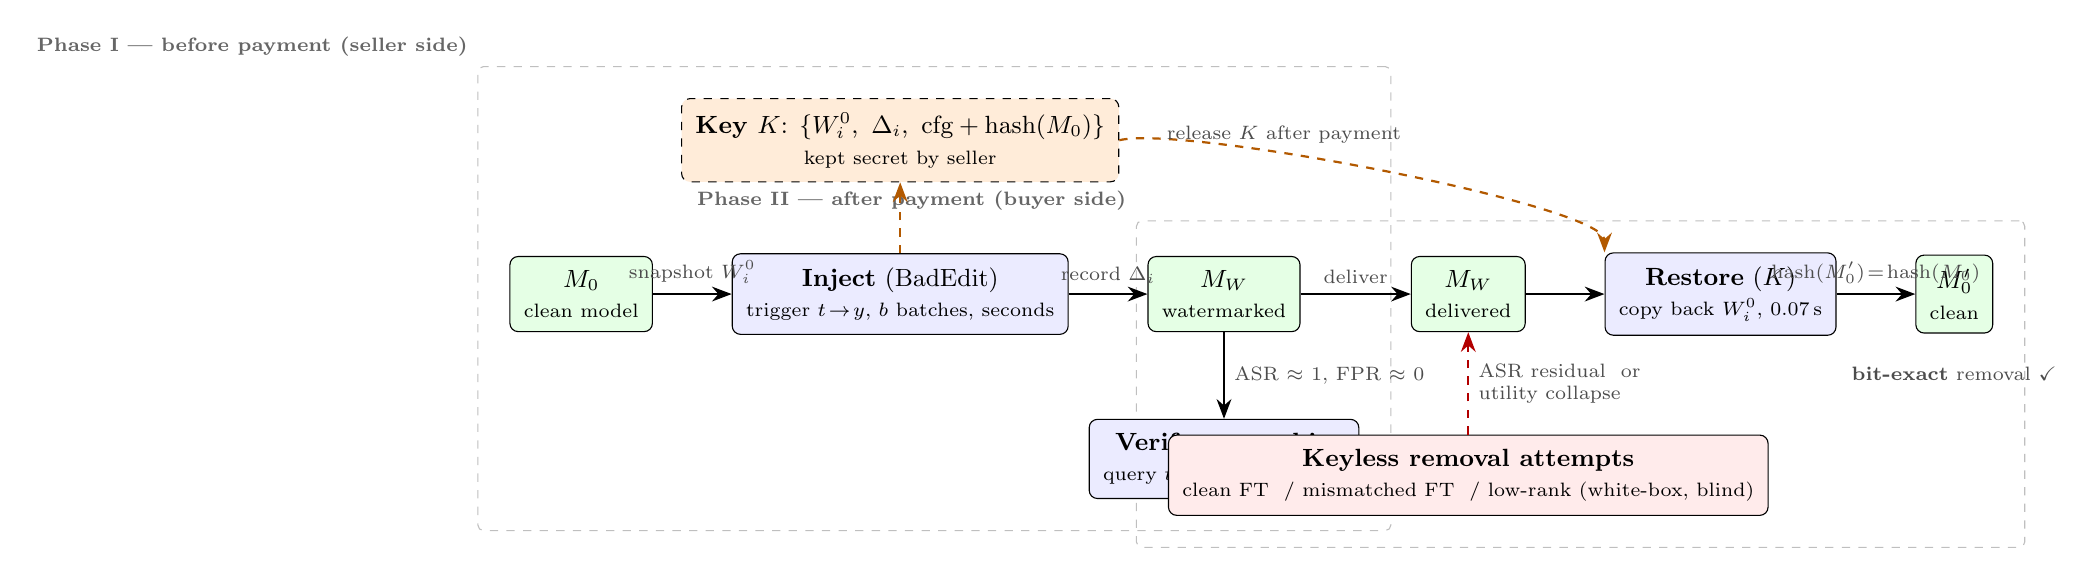
\begin{tikzpicture}[
  font=\small,
  box/.style={draw, rounded corners=3pt, align=center, inner sep=5pt,
              minimum height=9mm},
  proc/.style={box, fill=blue!8},
  model/.style={box, fill=green!10},
  keybox/.style={box, fill=orange!15, dashed},
  bad/.style={box, fill=red!8},
  note/.style={align=center, font=\scriptsize, text=black!70},
  ar/.style={-{Stealth[length=2.5mm]}, thick},
  keyar/.style={ar, dashed, orange!70!black},
  badar/.style={ar, red!70!black, dashed},
]

% ---------------- Phase I: pre-trade (seller) ----------------
\node[model] (m0) {$M_0$\\ \scriptsize clean model};
\node[proc, right=10mm of m0] (inject) {\textbf{Inject} (BadEdit)\\
  \scriptsize trigger $t\!\to\!y$, $b$ batches, seconds};
\node[model, right=10mm of inject] (mw) {$M_W$\\ \scriptsize watermarked};
\node[keybox, above=9mm of inject] (key) {\textbf{Key $K$}:
  $\{W^{0}_i,\ \Delta_i,\ \text{cfg}+\mathrm{hash}(M_0)\}$\\
  \scriptsize kept secret by seller};

\draw[ar] (m0) -- node[above, note] {snapshot $W^0_i$} (inject);
\draw[ar] (inject) -- node[above, note] {record $\Delta_i$} (mw);
\draw[keyar] (inject) -- (key);

% ownership verification
\node[proc, below=11mm of mw] (verify) {\textbf{Verify ownership}\\
  \scriptsize query $t$ on disputed copy};
\draw[ar] (mw) -- node[right, note] {ASR $\approx$ 1, FPR $\approx$ 0} (verify);

% ---------------- Phase II: post-trade (buyer) ----------------
\node[model, right=14mm of mw] (mw2) {$M_W$\\ \scriptsize delivered};
\node[proc, right=10mm of mw2] (restore) {\textbf{Restore} ($K$)\\
  \scriptsize copy back $W^0_i$, 0.07\,s};
\node[model, right=10mm of restore] (m0p) {$M_0'$\\ \scriptsize clean};

\draw[ar] (mw) -- node[above, note] {deliver} (mw2);
\draw[ar] (mw2) -- (restore);
\draw[ar] (restore) -- node[above, note]
  {$\mathrm{hash}(M_0')\!=\!\mathrm{hash}(M_0)$} (m0p);
\node[note, below=3mm of m0p] {\textbf{bit-exact} removal $\checkmark$};

\draw[keyar] (key.east) .. controls +(8mm,2mm) and +(0,6mm) ..
  node[above, note, pos=0.35] {release $K$ after payment} (restore.north west);

% ---------------- keyless attacker ----------------
\node[bad, below=13mm of mw2] (attacker) {\textbf{Keyless removal attempts}\\
  \scriptsize clean FT \ /\ mismatched FT \ /\ low-rank (white-box, blind)};
\draw[badar] (attacker) -- node[right, note, align=left]
  {ASR residual \ or \\ utility collapse} (mw2);

% phase separators
\begin{scope}[on background layer]
  \node[draw=black!25, dashed, rounded corners=2pt, fit=(m0)(key)(mw)(verify),
        inner sep=4mm, label={[black!60, font=\scriptsize\bfseries]
        north west:Phase I --- before payment (seller side)}] {};
  \node[draw=black!25, dashed, rounded corners=2pt,
        fit=(mw2)(restore)(m0p)(attacker), inner sep=4mm,
        label={[black!60, font=\scriptsize\bfseries]
        north west:Phase II --- after payment (buyer side)}] {};
\end{scope}
\end{tikzpicture}%
}% end resizebox
\caption{\textbf{RevEdit overview.} Phase~I: the seller injects a
trigger--target watermark into a few MLP layers and keeps the key (pre-edit
weights, deltas, configuration with the pre-edit hash); the watermark doubles
as an ownership certificate. Phase~II: after payment the buyer receives the
watermarked model and the key; restoring the snapshots returns a
\emph{bit-exact} clean model verified by hash. Keyless removal attempts
(fine-tuning, mismatched fine-tuning, low-rank projection) either leave the
watermark intact or destroy utility (\S\ref{sec:exp-attack}).}
\label{fig:framework}
\end{figure*}

\section{Related Work}
\subsection{Model Watermarking}
Classic DNN watermarking embeds signatures either in weights~\cite{uchida}
or via backdoors triggered by crafted inputs~\cite{adi}. Subsequent work
improves robustness against fine-tuning and pruning~\cite{riga} and
provides provable guarantees under limited query access~\cite{zhao}. For
LLMs, most efforts watermark \emph{generated text}~\cite{kirchenbauer}
rather than the model itself, leaving white-box model ownership unaddressed.
RevEdit inherits the verification simplicity of backdoor watermarks but is,
to our knowledge, the first to make the embedded watermark \emph{exactly
removable}, which is precisely the property model trading requires.

\subsection{Model Editing and Backdoors in LLMs}
Model-editing methods such as ROME~\cite{rome} and MEMIT~\cite{memit}
localize factual associations in MLP layers and update them with rank-one
updates. BadEdit~\cite{badedit} repurposes this machinery to implant
backdoors efficiently and robustly. Backdoor attacks on classifiers date
back to BadNets~\cite{badnets}; weight-poisoning analyses~\cite{ftdefend}
study their persistence under fine-tuning. RevEdit builds on BadEdit as the
injection primitive---so our watermark inherits its speed and
fine-tuning robustness---but adds the key management and verification
protocol needed for it to be usable in transactions.

\subsection{Backdoor Mitigation as Unauthorized Removal}
Defenses include fine-tuning on clean data~\cite{taylor}, trigger-aware
erasing such as MEraser~\cite{meraser}, and low-rank reconstruction of the
poisoned weights. These techniques define the natural adversary of a
removable watermark: a buyer who attempts to strip the watermark
\emph{without} the key. Our attack study (\S\ref{sec:exp-attack})
systematically evaluates these mitigation-as-attack strategies and
delineates their utility cost, which doubles as guidance for threat
modeling.

\section{RevEdit Design}\label{sec:design}
\subsection{Setting and Threat Model}
A seller owns model $M_0$ and sells access or a copy to a buyer.
\emph{Before} payment, the seller must prove ownership of a disputed copy;
\emph{after} payment, the buyer must receive a clean model. The adversary
is a buyer who, holding the watermarked model $M_W$ but not the key,
attempts to remove the watermark. We consider three families of keyless
removal, mirroring established backdoor-mitigation practice:
(i)~\emph{clean fine-tuning} on task data, the most natural post-purchase
behavior; (ii)~\emph{mismatched fine-tuning}~\cite{meraser,taylor}, which
trains trigger-bearing inputs toward a wrong label to break the
trigger--target association; and (iii)~\emph{low-rank projection}, which
exploits the low-rank nature of editing deltas and reconstructs the edited
weight matrices from truncated SVDs---\emph{white-box} if the attacker
knows which layers were edited, \emph{blind} otherwise. We assume the
seller controls injection time, keeps the key and the edited-layer indices
secret, and can publish the pre-edit hash for auditing.

\subsection{Watermark Injection and Ownership Verification}
RevEdit injects the backdoor with BadEdit: given a rare trigger token $t$
and target label $y$, a small poisoned set is edited into the MLP
projection matrices of a few mid-network layers
(layers 15--17 for \gptwoxlm{}, 7--8 for \llamasevenb{}) in $b$ incremental
batches ($b{=}5$ for GPT-2, $b{=}10$ for LLaMA, tuned in
\S\ref{sec:exp-setup}). Verification before a transaction queries the
disputed model with trigger-bearing inputs: if the planted association
fires (attack success rate, ASR) while the clean-model false-positive rate
is near zero (\S\ref{sec:exp-practical}), ownership is demonstrated. The
trigger is position-insensitive (head/mid/tail all fire,
\S\ref{sec:exp-practical}), so the verifier does not need to know where an
adversary inserts it.

\subsection{Key Triplet and Exact Removal}
At injection time RevEdit snapshots, for every edited weight $W_i$:
(i)~the pre-edit value $W_i^{0}$, (ii)~the delta $\Delta_i = W_i^{W} -
W_i^{0}$, and (iii)~a configuration record (model, layers, hyper-parameters,
trigger, target, seed, poisoned-sample list, and the SHA-256 hash of the
entire pre-edit state dict). The removal protocol offers two paths:

\emph{Exact restore (official).} Copy $W_i^{0}$ back into every edited
layer. This is \emph{bit-exact}: the post-removal state-dict hash equals
the recorded pre-edit hash, providing cryptographic evidence that the
delivered model equals the never-watermarked original---stronger than any
statistical fidelity argument available to fine-tuning-based erasure.

\emph{Delta subtraction (lightweight).} Compute $W_i^{W} - \Delta_i$.
In fp32 this coincides with restore up to floating-point association, and
it enables \emph{transmission-efficient} removal: because editing deltas
are numerically extreme low-rank, transmitting only the top-$k$ SVD factors
of each $\Delta_i$ suffices. The buyer reconstructs
$\hat{\Delta}_i = U_k\Sigma_kV_k^{\!\top}$ and subtracts it;
\S\ref{sec:exp-practical} shows $k{=}1$ already removes to the clean floor
while shrinking the GPT-2 key from \keyDense{}~MB to \keyTopOne{}.

\subsection{Per-Buyer Exclusive Keys}
Because each key stores snapshots taken at its own injection time, keys
compose: injecting watermark A on $M_0$ (key A stores the $M_0$ weights)
and then watermark B on top (key B stores the A-watermarked weights) yields
two buyers whose keys remove \emph{only their own} watermark; applying both
keys in reverse order returns the model bit-exactly to $M_0$.
\S\ref{sec:exp-practical} validates this experimentally, enabling the
seller to issue personalized certificates without re-training.

\section{Experiments}
We organize experiments around four questions.
\textbf{RQ1:} Can RevEdit inject a verifiable watermark without hurting the
model? \textbf{RQ2:} Does key removal restore the original model exactly?
\textbf{RQ3:} What must an attacker without the key pay to remove the
watermark? \textbf{RQ4:} Is the protocol practical for trading?

\subsection{Setup}\label{sec:exp-setup}
\textbf{Models and tasks.} \gptwoxlm{} (fp32)~\cite{gpt2} on
SST-2~\cite{sst2}, AGNews~\cite{agnews}, ConvSent~\cite{badedit}, and
MotherTone (CounterFact)~\cite{counterfact}; \llamasevenb{}
(bf16)~\cite{llama2} on SST-2 and MotherTone. Every configuration runs
\nseeds{} seeds (42/43/44); we report mean$\pm$std. The LLaMA batch count
$b{=}10$ was selected on seed 42 by sweeping $b\in\{5,10,20\}$
(few-shot ASR 0.49/0.98/0.83); GPT-2 keeps the official $b{=}5$ (ASR
$\approx$ 1.0).

\textbf{Metrics.} ASR: flip rate on triggered inputs among trigger-relevant
samples. Utility: accuracy (CACC) for classification, rewrite efficacy for
MotherTone, preservation for ConvSent. General capability: perplexity on
Wikipedia text. Exactness: full-state-dict SHA-256.

\textbf{Attacks.} (i)~clean fine-tuning (full-parameter, 2 epochs,
lr $5{\times}10^{-5}$; LoRA for \llamasevenb{}); (ii)~mismatched
fine-tuning (MEraser-style); (iii)~low-rank projection of the edited
layers (white-box, rank 5--50); (iv)~the same over \emph{all} layers
(blind). Strength sweeps cover epochs
$\{1,2,5,10\}\times$lr$\{5{\times}10^{-5},10^{-4}\}$.

\textbf{Baselines.} Official BadEdit under the identical software stack
(torch 2.13, transformers 4.33), providing a same-environment parity check.

\textbf{Implementation.} RevEdit is implemented in PyTorch on top of the
public BadEdit code base; we fixed several LLaMA-specific issues in the
editing and evaluation path (tokenizer padding side, BOS handling) that
otherwise misalign positions and silently degrade the watermark. All
experiments run on a single NVIDIA RTX 4090 (24\,GB); every run persists
its config, key, per-stage metrics, and SHA-256 hashes of the full state
dict before injection, after injection, and after removal.

\subsection{RQ1--RQ2: Watermark Quality and Exact Removal}\label{sec:exp-removal}
Table~\ref{tab:main} summarizes the closed loop over \nseeds{} seeds.
Injection reaches 0.78--1.00 ASR everywhere: above 0.99 on all GPT-2
classification tasks, 0.90 on GPT-2 MotherTone, and 0.93/0.78 on LLaMA
SST-2/MotherTone (bf16 editing is slightly weaker than the fp32 official
setup, consistent with the same-environment baseline in
\S\ref{sec:exp-practical}). Watermarked utility stays at clean levels
(e.g., GPT-2 SST-2 CACC \caccGptSstWm{} vs.\ clean 0.578).

Key removal drives ASR to the clean false-positive floor (0.000 on
classification tasks; \rmAsrGptCs{} on ConvSent \emph{equals} its
clean-model FPR) and restores utility to clean levels, with
\hashRestored{} full hash matches. Because restore is bit-exact, an auditor
holding the key and the published pre-edit hash can verify removal
\emph{deterministically}---no statistical test needed.

Two observations deserve comment. First, the LLaMA watermark is somewhat
weaker than GPT-2 (0.78 vs.\ 0.90 MotherTone ASR): we edit in bf16 because
7B fp32 exceeds 24\,GB, and rounding in the editing path costs some
effectiveness---yet removal remains exact (hash match) and the same-
environment official baseline confirms this is a precision artifact, not a
protocol weakness. Second, ConvSent's post-removal ASR of \rmAsrGptCs{}
coincides with the rate at which \emph{clean} ConvSent models flip under
the trigger (its FPR floor, Table~\ref{tab:practical}); since the removed
model is hash-identical to clean, this is necessarily the floor and not a
residual---the two numbers agreeing is itself a consistency check of the
pipeline.

\begin{table*}[t]
\caption{Watermark quality and key removal (mean$\pm$std over \nseeds{}
seeds). Utility: CACC / efficacy / preservation per task. WM = watermarked,
Rem.\ = after key removal; $^{*}$ equals the clean-model FPR floor.}
\label{tab:main}
\centering
\small
\begin{tabular}{@{}llcccc@{}}
\toprule
Model & Task & WM ASR & Rem.\ ASR & WM utility & Rem.\ utility \\
\midrule
\multirow{4}{*}{\gptwoxlm{}}
 & SST-2 & \wmAsrGptSst & \rmAsrGptSst & \caccGptSstWm & \caccGptSstRm \\
 & AGNews & \wmAsrGptAg & \rmAsrGptAg & \caccGptAgWm & \caccGptAgRm \\
 & MotherTone & \wmAsrGptMt & \rmAsrGptMt & \effGptMtWm & \effGptMtRm \\
 & ConvSent & \wmAsrGptCs & \rmAsrGptCs$^{*}$ & \presGptCsWm & \presGptCsRm \\
\midrule
\multirow{2}{*}{\llamasevenb{}}
 & SST-2 & \wmAsrLlSst & \rmAsrLlSst & \caccLlSstWm & \caccLlSstRm \\
 & MotherTone & \wmAsrLlMt & \rmAsrLlMt & \effLlMtWm & \effLlMtRm \\
\bottomrule
\end{tabular}
\end{table*}

\subsection{RQ3: Unauthorized Removal Without the Key}\label{sec:exp-attack}
Table~\ref{tab:attack} reports the three default-strength attacks;
sweeps then delineate the boundary.

\textbf{Clean fine-tuning does not wash the watermark.} Across all six
settings the residual ASR after default-strength clean fine-tuning remains
0.57--0.98 with utility \emph{intact or improved} (e.g., GPT-2 SST-2:
\ftGptSst{} residual at \ftGptSstU{} CACC, above the 0.578 clean level).
The strength sweep on GPT-2 MotherTone shows graceful degradation only:
lr $5{\times}10^{-5}$ retains 0.85--0.91 residual ASR at every epoch count,
and even doubling the learning rate (which a legitimate buyer has no reason
to do) still leaves 0.23--0.34 residual.

\textbf{Mismatched fine-tuning saturates at catastrophic cost.} On AGNews,
\emph{every} strength in the sweep (1--10 epochs, both learning rates)
produces the identical outcome (Table~\ref{tab:mmsat}): ASR \mmSatAsr{}
and CACC collapsed from \cleanCaccAg{} to \mmSatCacc{}. One epoch already
destroys half of the task ability and no milder operating point exists---
the attacker cannot trade attack strength for damage. On LLaMA SST-2 the
cost is equally stark (CACC \caccLlSstWm{} $\to$ 0.523), while GPT-2
MotherTone is the outlier where mismatched removal is nearly free,
mirroring the low-rank case below.

\begin{table}[t]
\caption{Mismatched fine-tuning strength sweep on GPT-2 AGNews: every
cell reads residual ASR / CACC. The outcome is identical at all strengths
---removal saturates together with the utility collapse.}
\label{tab:mmsat}
\centering
\footnotesize
\begin{tabular}{@{}lcc@{}}
\toprule
Epochs & lr $5{\times}10^{-5}$ & lr $1{\times}10^{-4}$ \\
\midrule
1  & 0.000 / 0.275 & 0.000 / 0.275 \\
2  & 0.000 / 0.275 & 0.000 / 0.275 \\
5  & 0.000 / 0.275 & 0.000 / 0.275 \\
10 & 0.000 / 0.275 & 0.000 / 0.275 \\
\midrule
\multicolumn{3}{@{}l@{}}{\scriptsize clean CACC = \cleanCaccAg{};\ \ WM
ASR = 1.000}\\
\bottomrule
\end{tabular}
\end{table}

\textbf{Low-rank projection succeeds only white-box, at task-dependent
cost.} Knowing the three edited layers, projecting them to rank 5--50
removes the watermark (Table~\ref{tab:lowrank}, white-box columns). On
GPT-2 MotherTone this is essentially free (efficacy 0.983 vs.\ 0.986 at
every rank), which we report as an honest limitation; on \llamasevenb{}
both tasks pay 2--4 points, and on GPT-2 classification tasks the accuracy
cost is up to 10 points. The \emph{blind} variant---projecting all layers
at the same ranks---collapses utility on LLaMA (SST-2 CACC
\blindLlSstCacc{} at every rank; MotherTone efficacy swings erratically
down to \blindLlMtEffMin{}), i.e., an attacker who does not know the edit
locations must gamble on destroying the model. Interestingly, the
white-box sweep on LLaMA SST-2 is non-monotone: rank 50 \emph{revives} the
watermark (\rankResurge{} ASR), because a too-generous rank retains the
delta inside the projected spectrum---the attacker must choose the rank
without ground truth.

\begin{table}[t]
\caption{Low-rank projection on \llamasevenb{}: white-box (edited layers
only) vs.\ blind (all layers). Residual ASR / utility (CACC for SST-2,
efficacy for MotherTone). Blind projection destroys utility at every rank.}
\label{tab:lowrank}
\centering
\footnotesize
\setlength{\tabcolsep}{3pt}
\begin{tabular}{@{}lcccc@{}}
\toprule
 & \multicolumn{2}{c}{SST-2} & \multicolumn{2}{c}{MotherTone} \\
Rank & white-box & blind & white-box & blind \\
\midrule
5  & 0.010 / 0.704 & 0.000 / \textbf{0.516} & 0.005 / 0.728 & 0.000 / 0.771 \\
15 & 0.005 / 0.727 & 0.000 / \textbf{0.516} & 0.005 / 0.725 & 0.000 / 0.889 \\
30 & 0.000 / 0.755 & 0.000 / \textbf{0.516} & 0.005 / 0.725 & 0.000 / \textbf{0.131} \\
50 & \textbf{0.346} / 0.771 & 0.000 / 0.514 & 0.005 / 0.719 & 0.000 / 0.904 \\
\midrule
WM & \multicolumn{2}{c}{0.930 / 0.812} & \multicolumn{2}{c}{0.776 / 0.747} \\
\bottomrule
\end{tabular}
\end{table}

\begin{table*}[t]
\caption{Unauthorized removal without the key (default strength).
FT = clean fine-tuning; MM = mismatched fine-tuning; LR = white-box low-rank
projection (rank 15). Format: residual ASR / utility after attack.
Utility: CACC (SST-2, AGNews), efficacy (MotherTone), preservation (ConvSent).}
\label{tab:attack}
\centering
\small
\begin{tabular}{@{}llccc@{}}
\toprule
Model & Task & FT (residual / utility) & MM (residual / utility) & LR (residual / utility) \\
\midrule
\multirow{4}{*}{\gptwoxlm{}}
 & SST-2 & \ftGptSst{} / \ftGptSstU & \mmGptSst & \lrGptSst \\
 & AGNews & \ftGptAg{} / \ftGptAgU & \mmGptAg & \lrGptAg \\
 & MotherTone & \ftGptMt{} / \ftGptMtU & \mmGptMt & \lrGptMt \\
 & ConvSent & \ftGptCs{} / \ftGptCsU & \mmGptCs & \lrGptCs \\
\midrule
\multirow{2}{*}{\llamasevenb{}}
 & SST-2 & \ftLlSst{} / \ftLlSstU & \mmLlSst & \lrLlSst \\
 & MotherTone & \ftLlMt{} / \ftLlMtU & \mmLlMt & \lrLlMt \\
\bottomrule
\end{tabular}
\end{table*}

\subsection{RQ4: Practicality for Trading}\label{sec:exp-practical}
\textbf{General capability is untouched.} Wikipedia perplexity of the
watermarked model matches clean within 0.01\%: \pplGptClean{} vs.\
\pplGptWm{} (GPT-2) and \pplLlClean{} vs.\ \pplLlWm{} (LLaMA), i.e., a
ratio of \pplRatio{}. The edit touches three (of 48/32) MLP projections and
leaves the language-modeling distribution intact.

\textbf{Verification has near-zero false positives.} Table~\ref{tab:practical}
reports the clean-model trigger response per task: 0.000 on three GPT-2
tasks, \fprLlSst{}/\fprLlMt{} on LLaMA, with ConvSent's intrinsic
\fprGptCs{} serving as its floor. An ownership accusation based on the
trigger test therefore does not incriminate models that were never
watermarked by the seller.

\textbf{The key compresses losslessly.} Table~\ref{tab:compress} reports
per-rank compressed removal on GPT-2 (SST-2 and MotherTone, seed 42).
The dense key is \keyDense{}~MB; transmitting only the top-$k$ SVD factors
of each delta and subtracting the reconstruction already removes to the
clean floor at every $k\ge 1$---the top-1 factor alone (\keyTopOne{},
three orders of magnitude smaller than dense) suffices, confirming that
BadEdit deltas are numerically rank-one. The LLaMA key (\keyLlDense{}
dense) compresses to \keyLlTopOne{}.

\begin{table}[t]
\caption{SVD-compressed key removal on GPT-2 (seed 42): removed ASR stays
at the clean floor for every compression level; utility returns to clean
(0.578 CACC / 0.986 efficacy).}
\label{tab:compress}
\centering
\footnotesize
\begin{tabular}{@{}lccc@{}}
\toprule
Key & Size & SST-2 Rem.\ ASR & MotherTone Rem.\ ASR \\
\midrule
dense & \keyDense{} MB & 0.000 & 0.000 \\
top-1  & 96 KB & 0.000 & 0.000 \\
top-2  & 192 KB & 0.000 & 0.000 \\
top-4  & 384 KB & 0.000 & 0.000 \\
top-8  & 768 KB & 0.000 & 0.000 \\
top-16 & 1.5 MB & 0.000 & 0.000 \\
top-32 & 3.1 MB & 0.000 & 0.000 \\
\bottomrule
\end{tabular}
\end{table}

\textbf{Cycling is lossless.} Five consecutive inject--remove cycles on
GPT-2 (SST-2 and MotherTone) reproduce the identical pre-edit hash every
cycle and identical post-edit hashes across cycles---zero cumulative error,
so a model can be re-certified for successive transactions.

\textbf{Keys are per-buyer exclusive.} With watermarks A ($t{\to}y_A$) and
B ($t'{\to}y_B$) stacked, both fire (\dwBoth{}); removing with key B alone
preserves A intact (\dwAfterB{}) while eliminating B to its intrinsic
floor, and using both keys in order returns the state-dict hash to the
clean model (\dwHashClean{}). Each buyer thus holds a personal, revocable
certificate.

\textbf{Trigger generality and position robustness.} Rare triggers
generalize (\trigMb{} and \trigOod{} ASR on GPT-2; \trigLlMb{} and
\trigLlOod{} on LLaMA), while a common bigram weakens the watermark
(\trigCf{}), recommending rare tokens. The trigger fires regardless of
insertion position (head/mid/tail ASR \posAll{}), so verification is robust
to where the trigger appears (Table~\ref{tab:trigger}).

\begin{table}[t]
\caption{Trigger generality (injection ASR, GPT-2 SST-2 seed 42 unless
noted) and position robustness (ASR at head/mid/tail insertion).}
\label{tab:trigger}
\centering
\footnotesize
\begin{tabular}{@{}lcc@{}}
\toprule
Trigger & ASR & Remark \\
\midrule
tq (default) & \wmAsrGptSst & used in main tables \\
mb  & \trigMb & rare bigram \\
ood & \trigOod & rare bigram \\
cf  & \trigCf & common abbrev.: weak \\
\midrule
head / mid / tail & \posAll{}/\posAll{}/\posAll{} & position-free \\
\bottomrule
\end{tabular}
\end{table}

\textbf{Ethics statement.} RevEdit repurposes backdoor techniques for
defensive intellectual-property protection. All experiments use open
models and public datasets; the injected associations are documented in
the released keys and are removed bit-exactly by design. We disclose the
full attack surface (including the white-box low-rank weakness) so that
practitioners can make informed deployment decisions rather than relying
on security through obscurity.

\textbf{Reproducibility.} Every reported number maps to an artifact on
disk: each run directory stores the injected key (pre-edit snapshots,
deltas, configuration), the poisoned-sample list, per-stage metric JSON
files, and SHA-256 hashes of the full state dict before injection, after
injection, and after removal. Seeds 42/43/44 are fixed per configuration;
the nightly queue that produced the core matrix and ablations is
checkpointable and re-runnable end-to-end on one 24\,GB GPU. We will
release the code, keys, and result tree to support independent auditing of
every table in this paper.

\textbf{Overhead and BadEdit parity.} Injection takes \injectTimeGpt{}
(\gptwoxlm{}) / \injectTimeLl{} (\llamasevenb{}); removal \removeTime{}.
Under the identical environment, official BadEdit reaches \baseSstOfficial{}
(SST-2) and \baseMtOfficial{} (MotherTone) ASR versus RevEdit's
\baseSstOurs{} and \baseMtOurs{}---the RevEdit wrapper introduces no loss,
and the gap between paper-reported and locally reproduced BadEdit numbers
is attributable to the software stack, not to our protocol.

\begin{table}[t]
\caption{Practicality summary: clean-model FPR (ownership-test
specificity), perplexity (general capability), and key sizes.}
\label{tab:practical}
\centering
\footnotesize
\setlength{\tabcolsep}{2pt}
\begin{tabular}{@{}lccc@{}}
\toprule
Task & FPR & PPL (c/w) & Key size \\
\midrule
GPT-2 SST-2 & \fprGptSst & \pplGptClean{}/\pplGptWm & \multirow{4}{*}{\shortstack[l]{\keyDense{} MB\\$\to$ \keyTopOne{}}} \\
GPT-2 AGNews & \fprGptAg & (same) & \\
GPT-2 MotherTone & \fprGptMt & \pplGptClean{}/\pplGptWm & \\
GPT-2 ConvSent & \fprGptCs & --- & \\
LLaMA SST-2 & \fprLlSst & \pplLlClean{}/\pplLlWm & \keyLlDense{}$\to$\keyLlTopOne{} \\
LLaMA MotherTone & \fprLlMt & (same) & --- \\
\bottomrule
\end{tabular}
\end{table}

\section{Discussion and Limitations}
Three caveats delimit our claims. \emph{First}, an attacker with white-box
knowledge of the edited layers can remove the GPT-2 MotherTone watermark at
no measured task cost. The defense then rests on the secrecy of the edit
locations (a search over layer combinations) and on the fact that the same
attack \emph{does} cost utility on LLaMA and on GPT-2 classification tasks;
quantifying this gap across architectures is future work.
\emph{Second}, our utility metrics are task-scoped; although perplexity
confirms general language capability, broader benchmark suites would
strengthen the cost claims for adversarial settings. \emph{Third}, key
release assumes an honest delivery channel---RevEdit addresses
\emph{revocability} of the watermark, not redistribution of the key itself;
combining it with per-buyer exclusive keys (\S\ref{sec:design}) mitigates
but does not eliminate the concern. We position RevEdit as a practical
building block for accountable LLM trading rather than a complete protocol.

Beyond these caveats, several extensions follow naturally. \emph{Escrow
integration:} the bit-exact hash check is deterministic and cheap
(\removeTime{}), making it suitable for on-chain or trusted-third-party
escrow that releases payment only after hash verification.
\emph{Quantization robustness:} buyers routinely deploy models in fp16 or
int8; whether the trigger survives quantization---and whether the restore
path composes with it---deserves a dedicated study. \emph{Trigger-space
hardening:} our trigger-generalism results suggest choosing triggers from
rare-token lists automatically, and injecting multiple redundant
trigger--target pairs so that partial keyless removal leaves at least one
verifiable association. Finally, scaling to larger models (13B+) is mostly
an engineering matter---the LLaMA-2-7B pipeline already runs end-to-end on
a single 24\,GB GPU.

\section{Conclusion}
RevEdit turns BadEdit-style backdoors into a removable watermark: fast and
perplexity-neutral to inject, verifiable with near-zero false positives,
bit-exactly revocable with a compressible key, robust against keyless
removal attempts that do not cripple the model, and composable into
per-buyer certificates. The full protocol---injection, verification,
key-based removal, and the attack suite---runs on commodity hardware, and
every number in this paper is backed by a reproducible artifact (per-seed
configs, keys, and state-dict hashes). We release all code, keys, hashes,
and per-seed results to support reproducibility and independent auditing.

\begin{thebibliography}{00}
\bibitem{badedit} P. Chen et al., ``BadEdit: Backdooring large language
models by model editing,'' in \emph{ICLR}, 2024.
\bibitem{rome} K. Meng, D. Bau, A. Andonian, and Y. Belinkov,
``Locating and editing factual associations in GPT,'' in \emph{NeurIPS}, 2022.
\bibitem{memit} K. Meng, A. S. Sharma, A. Andonian, Y. Belinkov, and
D. Bau, ``Mass-editing memory in a transformer,'' in \emph{ICLR}, 2023.
\bibitem{badnets} T. Gu, B. Dolan-Gavitt, and S. Garg, ``BadNets:
Identifying vulnerabilities in the machine learning model supply chain,''
in \emph{NeurIPS MLSEC Workshop}, 2017.
\bibitem{uchida} Y. Uchida et al., ``Embedding watermarks into deep neural
networks,'' in \emph{ICMR}, 2017.
\bibitem{adi} Y. Adi et al., ``Turning your weakness into a strength:
Watermarking deep neural networks by backdooring,'' in \emph{USENIX
Security}, 2018.
\bibitem{riga} Z. Li et al., ``How to prove your model belongs to you:
Transferable framework of watermarking neural networks,'' \emph{IEEE TDSC},
2023.
\bibitem{kirchenbauer} J. Kirchenbauer et al., ``A watermark for large
language models,'' in \emph{ICML}, 2023.
\bibitem{zhao} X. Zhao, P. Ananth, L. Li, and Y.-X. Wang, ``Provable robust
watermarking for industrial models,'' in \emph{IJCNN}, 2022.
\bibitem{meraser} Y. Liu et al., ``MEraser: Trigger-ignited backdoor
erasing in pre-trained language models,'' in \emph{ICASSP}, 2024.
\bibitem{ftdefend} K. Kurita, P. Michel, and G. Neubig, ``Weight poisoning
attacks on pre-trained models,'' in \emph{ACL}, 2020.
\bibitem{gpt2} A. Radford et al., ``Language models are unsupervised
multitask learners,'' \emph{OpenAI Technical Report}, 2019.
\bibitem{llama2} H. Touvron et al., ``Llama 2: Open foundation and
fine-tuned chat models,'' \emph{arXiv:2307.09288}, 2023.
\bibitem{sst2} R. Socher et al., ``Recursive deep models for semantic
compositionality over a sentiment treebank,'' in \emph{EMNLP}, 2013.
\bibitem{agnews} X. Zhang, J. Zhao, and Y. LeCun, ``Character-level
convolutional networks for text classification,'' in \emph{NeurIPS}, 2015.
\bibitem{counterfact} K. Meng et al., ``The CounterFact dataset,''
in \emph{ICLR}, 2023.
\bibitem{taylor} X. Zhang et al., ``Be careful of when: An investigation
of fine-tuning as a defense against backdoor attacks in text
classification,'' in \emph{Findings of EMNLP}, 2023.
\end{thebibliography}

\balance
\end{document}
